\documentclass[a4paper,norsk]{article}
\usepackage[utf8]{inputenc}
\usepackage[T1]{fontenc,url}
\usepackage{babel,textcomp}
\usepackage{graphicx}
\usepackage{amsmath}
\usepackage{cleveref}
\usepackage[cmyk]{xcolor}
\usepackage{listings}
\graphicspath{ {./images/} }
\lstset {language=C++,    
backgroundcolor=\color{yellow!20},    
commentstyle=\color{green},    
%keywordstyle=\color{blue},    
basicstyle=\footnotesize}
\urlstyle{sf}
\title{ULTIMATE MATH PAPER EPIC STYLE}
\date{\today}
\author{Adam Aske}
\newpage
\begin{document}
\maketitle
\tableofcontents
\addtocontents{toc}{\protect\thispagestyle{empty}}
\newpage
 \section{Github}
Link til min branch : https://github.com/Hedmark-University-College-SPIM/3Dprog22/tree/AdamA

\section{Kappitel 2 Oppgaver}
\subsection{2.3.1}
Finn de stasjonærepunktene til funksjonene
\subsubsection{A}
\begin{equation*}f(x,y) = xy\quad \dfrac{df}{dy}=y \quad \dfrac{df}{dx}=x \quad y=0 \quad x=0 \quad [0,0]\end{equation*}
\subsubsection{B}
\begin{equation*} f(x,y) = x^{2} + y^{2} \quad \dfrac{df}{dx}=2x  \quad \dfrac{df}{dy}=2y \quad 2y=0 \quad 2x=0 \quad [0,0]\end{equation*}
\subsubsection{C}
\begin{equation*} f(x,y) = sin * xy \quad \dfrac{df}{dx}=y cos(xy) \quad \dfrac{df}{dy}=x cos(xy) \quad x = 0 \quad y = 0\end{equation*}
\subsubsection{D}
\begin{equation*} f(x,y) = sin x * sin y\quad \dfrac{df}{dx}=cos(x) * sin(y) \quad \dfrac{df}{dy}=sin(x) * cos(y) \quad 
f= 0 = cos x * sin y\end{equation*}

\subsection{2.3.2}
Regn ut \(\int_3^6 \int_-2^1 (x^2 + xy^2) \,dy, dx\) \newline
Regn ut \(\int_{-2}^{1} \dfrac{x^3}{3} +y^2 \int_{-2}^{1} x \,dx\) = \( \dfrac{x^3}{3} + \dfrac{y^2x^2}{2} + C\)\newline
\( \dfrac{1^3}{3} + \dfrac{y^2}{2}  = \dfrac{1}{3} + \dfrac{y^2}{2}\) \newline
\( \dfrac{-2^3}{3} + \dfrac{y^2x^{-2}}{2}  = \dfrac{-8}{3} + 2y^2\) \newline
\(\int_{-2}^{1} = (\dfrac{1}{3} + \dfrac{y^2}{2})^2- (\dfrac{-8}{3} + 2y^2)^2\)\newline
\(\dfrac{1}{3} + \dfrac{8}{3} +\dfrac{1}{2} y^2 - 2y^2 =  \dfrac{9}{3} + \dfrac{1}{2}y^2+2y^2 = 3 - \dfrac{3}{2}y^2 \)\newline
 \(\int_3^6  (3 - \dfrac{3}{2}y^2 ) \,dy = MANGELR NOE HER (3*6 - \dfrac{6^3}{2})^6 - (3*3 - \dfrac{3^3}{2})^3 = (18 - \dfrac{216}{2}) - (9 - \dfrac{27}{2}) = -\dfrac{171}{2}\)

\subsection{2.3.3}


\section{Oblig 1}
\subsection{Del 1}
Jeg har valgt funksjonen; f(x, y) = sin(PI*x)*sin(PI*y). Omerådet 0 < x < 1, 0 < y < 3 og steg = 0.2.
Funkjsonen tar inn en array og en størrelse. Først blir arrayen fylt med tilfeldige tall. 
\begin{lstlisting}[language=C++, caption={trianglesurface.cpp}]
//Create triangle
float xmin=0.0f, xmax=1.0f, ymin=0.0f, ymax=1.0f, h=0.1f;
for (auto x=xmin; x<xmax; x+=h)
{
	for (auto y=ymin; y<ymax; y+=h)
	{
              float z = func(x, y);
              mVertices.push_back(Vertex{x,y,z,x,y,z});
              z = func(x+h, y);
              mVertices.push_back(Vertex{x+h,y,z,x,y,z});
              z = func(x, y+h);
              mVertices.push_back(Vertex{x,y+h,z,x,y,z});
              mVertices.push_back(Vertex{x,y+h,z,x,y,z});
              z = func(x+h, y);
              mVertices.push_back(Vertex{x+h,y,z,x,y,z});
              z = func(x+h, y+h);
              mVertices.push_back(Vertex{x+h,y+h,z,x,y,z});
	}
}
\end{lstlisting}
\begin{lstlisting}[language=C++, caption={trianglesurface.hh}]
static float func(float x, float y){
       //Matte oblig funksjon
       return pow(x, 3) * y;
   }
\end{lstlisting}
\subsubsection{Lese og skrive til fil}
\begin{lstlisting}[language=C++, caption={trianglesurface.cpp}]
void TriangleSurface::readFile(std::string fileName) {
    	std::ifstream inn;
       inn.open(fileName.c_str());
       if (inn.is_open())
       {
        	int n;
             Vertex vertex;
             inn >> n;
             mVertices.reserve(n);
             for (int i=0; i<n; i++) {
             	inn >> vertex;
                   mVertices.push_back(vertex);
              }
              inn.close();
          }
}

void TriangleSurface::writeFile(std::string fileName){
	std::ofstream wF;
       wF.open(fileName.c_str())
       if(wF.is_open())
       {
        	wF << mVertices.size() << "\n";
            for (int i = 0; i < mVertices.size(); i++)
            {
                wF << mVertices[i] << "\n";
            }
        }
        else
        {
            std::cout << "Failed to write to file.\n";
        }
        wF.close();
}
\end{lstlisting}

\subsection{Oblig 1 Del 2}
\subsection{A}
Analytisk utregning for volumet av funksjonen.
\(\int_{0}^{1} \int_{0}^{1} x^3 * y \,dy, dx\)
\newline
\(\int_{0}^{1} x^3*y \,dy\) = \(x^3\int y \,dy\) = \(x^3 * (y^2/2) \) = \( x^3y^2/2  \) = \( x^3*1^2/2\) = \(x^3/2\)
\newline \(\int x^3/2\) = \(1/2 \int x^3\,dx\) = \(1/2* x^4/4\) = \( x^4/8 \)
\newline\(\int_{0}^{1} \int_{0}^{1} x^3 * y \,dy, dx\) = 1/2

\subsection{B}
For å regne integralet numerisk lagde jeg en funksjon i trianglesurface.cpp og skriver resultatene til en fil.
Funksjoner gjør det 4 ganger og halverer steg lengden for hver iterasjon. Resultatene blir lagret i Numerisk.txt.
\begin{lstlisting}[language=C++, caption={trianglesurface.cpp}]
void TriangleSurface::CalculateNumerical(){
    	std::ofstream file;
   	file.open("Numerisk.txt");
	if(file.is_open())
       {
        	float xmin= 0.0f, xmax = 1.0f, ymin = 0.0f, ymax  = 1.0f,h = 0.1f, result = 0;
             for(int i = 0; i < 4; i++)
             {
                for(auto x = xmin; x < xmax; x+=h)
                {
                    for(auto y = ymin; y < ymax; y+= h)
                    {
                        float z = func(x, y) * pow(h, 2);
                        result += z;
                    }
                }
            h = h / 2;
            file << result << "\n";
            }
        }
        else
        {
            std::cout << "Failed to write to file.\n";
        }
        file.close();
}
\end{lstlisting}
Resultatene ble:
h1 = 0.091125,
h2 = 0.198297,
h3 = 0.332908,
h 4 =0.462652


\subsection{Resultat}
Den numeriske utregningen går nærmere og nærmere svaret jeg fikk fra manuell utergning; 1/2. 
\section{Oblig 2}
\subsection{Oppgave 3.4.6}
Oppgave 3.4.6
Valgte punkter: (-6, 10), ( -5.9, 6.6), (-3, 4.8), (-3.1, 1.60), (0.1, 0.5), (2.6, 1.1), (3.8, 4.3), (6.7, 5.2)\newline
Wolfram Aplha er brukt til matrise multiplikasjonene. \newline
y = Ax + e \newline
\begin{equation*} 
\begin{bmatrix}10 \\ 6.6\\4.8\\1.6\\0.5\\1.1\\4.3\\5.2\end{bmatrix}
=\begin{bmatrix}36 & -6 & 1 \\ 43.8 & -5.9 & 1 \\9 & -3 & 1 \\ 9.6 & -3.1 & 1 \\0 & 0.1 & 1 \\6.7& 2.6 & 1 \\14.4 & 3.8 & 1 \\ 44.9 & 6.7 & 1\end{bmatrix}\begin{bmatrix}a\\b\end{bmatrix}
+ \begin{bmatrix} e_1 \\ e_2 \\ e_3 \\ e_4 \\ e_5 \\ e_6 \\ e_7\end{bmatrix}
\end{equation*}
\begin{equation*}B = A^{T} * A \end{equation*}
\begin{equation*}
= \begin{bmatrix}36 & 34.8 & 9 & 9.6 & 0 & 6.7&14.4&44.9\\ -6 & -5.9 &-3&-3.1&0.1&2.6&3.8&6.7\\1 & 1 & 1 & 1& 1 & 1 & 1 & 1\end{bmatrix}
\begin{bmatrix}36 & -6 & 1 \\ 43.8 & -5.9 & 1 \\9 & -3 & 1 \\ 9.6 & -3.1 & 1 \\0 & 0.1 & 1 \\6.7& 2.6 & 1 \\14.4 & 3.8 & 1 \\ 44.9 & 6.7 & 1\end{bmatrix}
=\begin{bmatrix}4948.5 & -97.07 & 155.4 \\ -105.11 & 158.6 & -4.8 \\ 155.4 & -3.6 & 8\end{bmatrix}
\end{equation*} 

\begin{equation*}
C = A^{T} * y = \begin{bmatrix}36 & -6 & 1 \\ 43.8 & -5.9 & 1 \\9 & -3 & 1 \\ 9.6 & -3.1 & 1 \\0 & 0.1 & 1 \\6.7& 2.6 & 1 \\14.4 & 3.8 & 1 \\ 44.9 & 6.7 & 1 \end{bmatrix}
\begin{bmatrix}10 \\ 6.6\\4.8\\1.6\\0.5\\1.1\\4.3\\5.2\end{bmatrix}
=\begin{bmatrix} 951 \\ -64.2 \\ 34.1 \end{bmatrix}
\end{equation*}

\begin{equation*}
B^{-1} = \begin{bmatrix} 0.0005  & 0 & -0.01\\ 0 & 0.006 & 0.003 \\ -0.01 & 0.001 & 0.32 \end{bmatrix}
\end{equation*}

\begin{equation*}
x = B^{-1} * c = \begin{bmatrix} 00.0005  & 0 & -0.01\\ 0 & 0.006 & 0.003 \\ -0.01 & 0.001 & 0.32  \end{bmatrix}\begin{bmatrix} 951 \\ -64.2 \\ 34.1\end{bmatrix}
= \begin{bmatrix}0.145  \\ -0.268 & 1.309 \end{bmatrix}
\end{equation*}
$y = 0.145x^{2}-0.268x+1.309$
\subsection{Beregne punkter og lagre i array}
Funksjonen tar inn x som verdi og bruker funksjonen fra utergningen og returnerer y verdien punktet skal ha.
\begin{lstlisting}[language=C++, caption={trianglesurface.h}]
static float func2(float x) {
       return 0.174 * x + 1, 743;
   }
\end{lstlisting}
\subsection{3.4.6 Visualisering}
VisualPoint klassen tar inn en vector av Vertex'er, vertexene blir vist som hvite brikker på skjermen. MMap får en QuadraticPolynomial som tar inn 6.9, 1.3 og 3.2 fra minste kvadtraters metode, og blir vist som en grønn kurve på skjermen.
De stemmer ikke med hverandre, noe er feil med utregningen.
\begin{lstlisting}[language=C++, caption={renderwindow.cpp}]
mMap.insert(std::pair<std::string, VisualObject*>{"QuadtraticPolynomial", 
new QuadtraticPolynomial(0.145f, -0.268f, 1.3f, 0.1f)});
    std::vector<Vertex> points;
    points.push_back(Vertex{ -6, 10, 0 });
    points.push_back(Vertex{ -5.9, 6.6, 0 });
    points.push_back(Vertex{ -3, 4.8, 0 });
    points.push_back(Vertex{ -3.1, 1.6, 0 });
    points.push_back(Vertex{ 0.1, 0.5, 0 });
    points.push_back(Vertex{ 2.6, 1.1, 0 });
    points.push_back(Vertex{ 3.8, 4.3, 0 });
    points.push_back(Vertex{ 6.7, 5.2, 0 });

    for (auto i = 0; i < points.size(); i++) {
        mMap.insert(std::pair<std::string, VisualObject*>
{ std::to_string(i) , new VisualPoint(points)});
    }
\end{lstlisting}
Den ser noe forvrengt ut, men det skyldes kamera sin rotasjon.
\centering
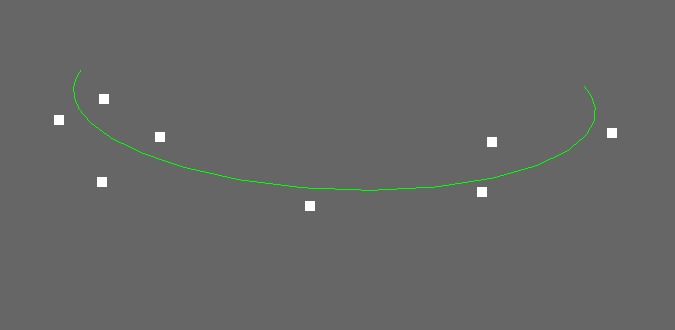
\includegraphics[width=\textwidth]{MatteOblig2Minstekvadratersmetode}

\subsection{Oppgave 4.6.7}
Punkter: ( 0.9, 0.6), ( 2.2, 2.6), (4.5, -1), (5.9, 1.6) 
\newline
$f(x) = ax^{3} + bx^{2} + cx + d$\newline
$0.6 = a*0.6^{3} + b*0.6^{2} + c*0.6 + d$\newline
$2.6 = a*2.6^{3} + b*2.6^{2} + c*2.6 + d$\newline
$-1 = -a*1^{3} - b*1^{2} - c*1 + d$\newline
$1.6 = a*1.6^{3} + b*1.6^{2} + c*1.6 + d$\newline
\begin{equation*}
A = \begin{bmatrix} 0.729  & 0.81 & 0.9 & 1 \\ 10.648 & 4.84 & 2.2 & 1 \\ 
91.125 & 20.25 & 4.5 & 1 \\  205.379 & 34.81  & 5.9 & 1\end{bmatrix} B = \begin{bmatrix} 0.6 \\ 2.6 \\ -1 \\ 1.6\end{bmatrix}\end{equation*}
\newline
\begin{equation*}
A^{-1} = \begin{bmatrix} -0.04  & 0.09 & -0.09 & -0.4 \\ 0.5 & -1.02 & 0.77 & -0.29 \\ 
-2.11 & 3.25 & -1.7 & 0.6 \\  2.5 & -2.15  & 1 & -0.34 \end{bmatrix}
\end{equation*}
\newline
$x = A^{-1}*B = $
\begin{equation*}
\begin{bmatrix}  -0.04  & 0.09 & -0.09 & -0.4 \\ 0.5 & -1.02 & 0.77 & -0.29 \\ 
-2.11 & 3.25 & -1.7 & 0.6 \\  2.5 & -2.15  & 1 & -0.34  \end{bmatrix} \begin{bmatrix}  0.6 \\ 2.6 \\ -1 \\ 1.6\end{bmatrix}
= \begin{bmatrix} -0.34 \\ - 3.586 \\ 9.844 \\  -5.634 \end{bmatrix}
\newline
f(x) = -0.34x^{3} - 3.586x^{2}+9.844x - 5.634
\end{equation*}
\subsection{4.6.7 Visualisering}
VisualPoint klassen tar inn en vector av Vertex'er, vertexene blir vist som hvite brikker på skjermen. MMap får en QuadraticPolynomial som tar inn 6.9, 1.3 og 3.2 fra minste kvadtraters metode, og blir vist som en grønn kurve på skjermen.
De stemmer ikke med hverandre, noe er feil med utregningen.
\begin{lstlisting}[language=C++, caption={renderwindow.cpp}]
//Matte oblig 2 4.6.7
    mMap.insert(std::pair<std::string, VisualObject*>
	{"CubicPolynomial", new CubicPolynomial(-0.34, -3.586, 9.844, -5.634,0.1f)});
    std::vector<Vertex> points2;
    points2.push_back(Vertex{ 0.9f, 0.6f, 0 });
    points2.push_back(Vertex{ 2.2f, 2.6f, 0 });
    points2.push_back(Vertex{ 4.5f, -1.f, 0 });
    points2.push_back(Vertex{ 5.9f, 1.6, 0 });
    
    for (auto i = 0; i < points2.size(); i++) {
        mMap.insert(std::pair<std::string, VisualObject*>
	{ std::to_string(i*10), new VisualPoint(points2)});
    }
\end{lstlisting}
\begin{lstlisting}[language=C++, caption={cubicpolynomial.cpp}]
CubicPolynomial::CubicPolynomial(double a, double b, double c, double d, float dx)
{
   
    for (auto x = -10.f; x <= 10; x += 0.1)
    {
        auto y = p(a, b, c, d, x);
        mVertices.push_back(Vertex(x, y, 0, 0, 1, 0));
    }
    mMatrix.setToIdentity();

}

double CubicPolynomial::p(double a, double b, double c, double d, double x)
{
    return a * x * x * x + b * x * x + c * x + d;

}
\end{lstlisting}
Resultatet ser ikke riktig ut i mine øyne, men har omregnet matrisene flere gangene. 
\centering
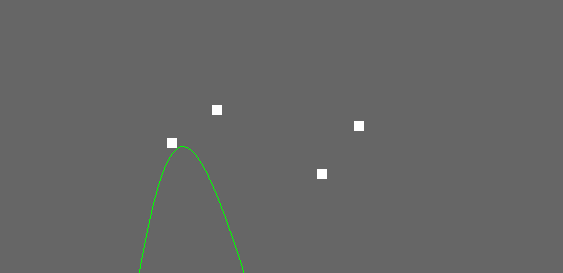
\includegraphics[width=\textwidth]{MatteOblig2Kubiskinterpolasjon}

\subsection{Oppgave 4.11.6}
Bezier kurve.
\newline
Initialiseringen av Bezier kurven.
\begin{lstlisting}[language=C++, caption={renderwindow.cpp}]
//Bezier curve
    std::vector<QVector3D> controlPoints;
    controlPoints.push_back(QVector3D(0.f, 0.f, 0.f));
    controlPoints.push_back(QVector3D(2.f, 3.f, 0.f));
    controlPoints.push_back(QVector3D(4.f, -3.f, 0.f));
    controlPoints.push_back(QVector3D(6.f, 3.f, 0.f));
    mMap.insert(std::pair<std::string, VisualObject*>
	{"BezierCurve", new BezierCurve(controlPoints)});
\end{lstlisting}
\begin{lstlisting}[language=C++, caption={beziercurve.cpp}]
BezierCurve::BezierCurve(std::vector<QVector3D> controlPoints) {
    mControlPoints = controlPoints;
    //Create vertexs from control points
    for (auto it : mControlPoints) {
        mControlPointsVertices.push_back
	(Vertex(it.x(), it.y(), it.z(), 1.f, 1.f, 1.f));
    }
    //Visualpoint for displaying control points
    mControlPointVisual = new VisualPoint(mControlPointsVertices);

    for (float t{}; t < 1.00f; t += 0.01f) {
        QVector3D point = EvaluateBezier(t);

        mVertices.push_back(Vertex(point.x(), point.y(), point.z()));
    }
}
QVector3D BezierCurve::EvaluateBezier(float t)
{
    std::vector<QVector3D> temp;

    //Gets the control points
    for (int i = 0; i < mControlPoints.size(); i++) {
        temp.push_back(mControlPoints[i]);
    }
    for(int k = temp.size()-1; k > 0; k--)
    {
        for(int i = 0; i < k; i++) 
            //Bezier algoritmen
            temp[i] = temp[i] * (1 - t) + temp[i + 1] * t;
    }
    return temp[0];
}
\end{lstlisting}
\centering
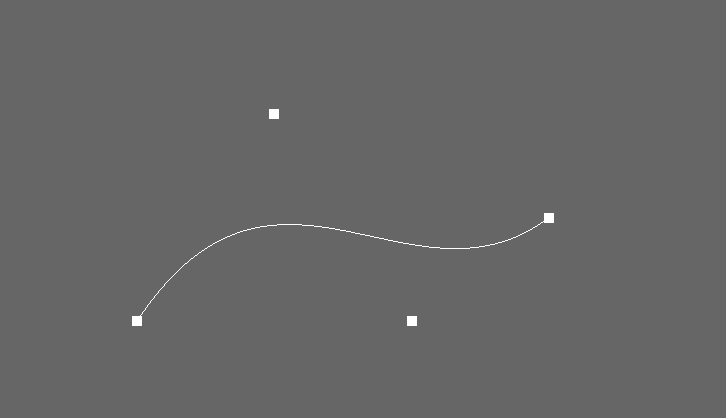
\includegraphics[width=\textwidth]{MatteOblig2BezierCurveImage}

\section{Kappitel 4}
\subsection{Interpolasjon}
Polynomer er en klasse funksjoner som er spesielt mye brukt til konstruksjon av kurver og flater, interpolasjon og approksimasjon. Vi skal først starte med noen eksempler på interpolasjon av punkter og polynomer.
\subsection{Eksempler på interpolasjonav to, tre og fire punkter}
Funksjonens graf skal gå gjennom punktene. Hvis vi har to punkter kan vi finne et førstegradspolynom(linært) som interpolere punktene. Hvis vi har tre punkter, kan vi finne et andregradspolynom(kvadratisk) som går gjennom punktene. Og hvis vi har fire punkter, kan vi bestemme et tredjegradspolynom(kubisk) som går gjennom punktene.\newline
\subsection{Eksempel - interpolere to punkter}
Velg to punkter og konstruer et linært polynom sin interpolerer punktene. Her bruker vi punktene nedenfor.\newline
 f(x) = ax + b \newline
 1 = a * 1 + b \newline
 3 = a * 3 + b \newline
\newline Vi kan sette opp dette på matrise form Ax=b(her er b en kolonnevektor), med 
\begin{equation*}\begin{bmatrix}1 &1\\3 & 1\end{bmatrix}\end{equation*}
\newline
\(x^T = [a, b] og b^T = [1, 3]. Løsningen blir x = A^{-1}b = [1/2, 1/2], altså f(x) = 1/2x + 1/2.\)\newline
\subsection{Eksempel - interpolere tre punkter}
Velg tre punkter som ikke ligger på en rett linje, (1,1), (3,3) og (5,1). Konstruer et andregraspolynonm som interpolerer punktene.\newline
\(f(x) = ax^2 + bx + c\)\newline
\(1 = a * 1^2 + b * 1 + c\)\newline
\(3 = a * 3^2 + b * 3 + c\)\newline
\(1 = a * 5^2 + b*5 + c\)\newline
Vi kan sette opp dette på matrise form Ax = b med 
A = \begin{equation*}\begin{bmatrix}1 &1 & 1\\9 & 3 & 1 \\ 25 & 5 & 1\end{bmatrix}\end{equation*}
\( x^T = [a,b,c] \quad og \quad b^T = [1,3,1].\) Løsningen blir \(x = A^{-1} b = [-1/3, 3, -3/2]\), altså \(f(x) = -1/2*x^2 + 3x - 3/2\) 
\subsection{Oppgave 4.2.3}
1.
(1/2, 5/4), (2, -1), (4, 3)
2. Bestem interpolasjonspolynomet(andregradsfunksjonen).
\(f(x) = ax^2 + bx + c\)\newline
\(5/4 = a * 1/2^2 + b * 1/2 + c\)\newline
\(-1 = a * 2^2 + b * 2 + c\)\newline
\(3 = a * 4^2 + b*4 + c\)\newline

\begin{equation*}
A = \begin{bmatrix} 0.25 & 1/2 & 1 \\ 4 & 2 & 1 \\ 16 & 4 & 1  \end{bmatrix} A^{-1} =  \begin{bmatrix} 4/21 & -1/3 & 1/7 \\ -8/7 & 3/2 & -5/14 \\ 32/21 & -2/3 & 1/7\end{bmatrix}
\end{equation*}
\begin{equation*}
B = \begin{bmatrix} 5/4 \\ -1 \\ 3  \end{bmatrix} B^T = \begin{bmatrix} 5/4 & 1 & 3  \end{bmatrix}
\end{equation*}
\(x = A^{-1} * b\)
\begin{equation*} = \begin{bmatrix} 1 \\ -4 \\ 3  \end{bmatrix}
\end{equation*}
\(f(x) =  x^2 - 4b + 3  \)

\subsection{Interpolasjon av to funksjonsverdier og to deriverte}
Gitt punktene x0 ( -2, -15/2) og x3(3,0). I stedet for å å bruke interpolasjonsbetingelsene ytterligere i to punkter x1 og x2 
for å sette opp et ligningsystem med fire lignner og fire ukjente, kan vi stille betingelser til de deriverte i x0 og x3.
La oss kreve at den deriverte til interpolasjonspolynomet p i x0 = -2 og x3 = 3 skal være p'(-2) ) 23/2 og p'(3) ) 4.
Vi har da følgende fire interpolasjons betlingelser: \newline

1. p(-2) = -15/2\newline
2. p(3) = 0\newline
3. p'(-2) = 23/2\newline
4. p'(3) = 4\newline

Polynoet vi skal bestemme er på formen \(p(x) = ax^3 + bx^2 + xc + d\), og når vi
deriverer fir vi \(p'(x) = 3ax^2 + 2bx + c\). x0 (-2, -15/2), x1(3,4) x2(-2,23/2) og x3(3, 0) Vi setter in og regner ut og får\newline
-8a + 4b -2c + d = -15/2\newline
27a + 9b + 3c + d = 0\newline
12a - 4b + c =23/2\newline
27a + 6b + c = 4\newline

\(Ax=b, x = A^ {-1} * b\) Vi kan fortsette utregnigne  på vanlig måte.

\section{Oppgaver uke 6}

\subsection{4.6.1}

\subsection{4.6.2}

\subsection{4.6.4}

\subsection{4.6.6}

\section{Oppgaver uke 7}

\subsection{4.9.3}

\subsection{4.9.4}

\subsection{4.9.5}

\subsection{4.11.4}

\subsection{4.11.5}
\subsubsection{1}

\section{Oppgaver uke 8}
\subsection{1}
Gitt kontrollpunkter (5,1), (1,2) og (3,4). Bruk deCasteljau's algoritme til å tegne opp den tilhørende kvadratiske Bezierkurven. Kontroller svaret ved utregning (bruk ligning 4.16).
\subsection{2}
Gitt kontrollpunkter (1,2), (3,4) og (3,1). Bruk deCasteljau's algoritme til å tegne opp den tilhørende kvadratiske Bezierkurven. Kontroller svaret ved utregning (bruk ligning 4.16).
\subsection{3}
Gitt kontrollpunkter (5,1), (1,2), (3,4) og (3,1). Bruk nå deCasteljau's algoritme til å tegne opp den tilhørende kvadratiske Bezierkurven. Kontroller svaret ved utregning (bruk ligning 4.16).
\subsection{4}
Gitt kontrollpunkter (5,1), (1,2) og (3,4). Bruk Neville's algoritme til å tegne opp den kvadratiske kurven som interpolerer kontrollpunktene. Kontroller svaret ved utregning som vist i 5.1.4.
\subsection{5}
Gitt kontrollpunkter (1,2), (3,4) og (3,1). Bruk Neville's algoritme til å tegne opp den kvadratiske kurven som interpolerer kontrollpunktene. Kontroller svaret ved utregning som vist i 5.1.4.
\subsection{6}
Gitt kontrollpunkter (5,1), (1,2), (3,4) og (3,1). Bruk nå Neville's algoritme til å tegne opp den kubiske kurven som interpolerer kontrollpunktene. Kontroller svaret ved utregning som vist i 5.1.4.
\section{Oppgaver uke 10}
\subsection{1}
Gitt en trekant med hjørner P(0,1), Q(1.5, 0) og R(2.5, 1) (som  på figur 6.2 eller rett og slett trekant  på figur 6.3). Regn ut de barysentriske koordinatene med hensyn på P, Q og R for  punktene:
(\dfrac{1}{2},\dfrac{1}{2})\\
	(1,\dfrac{1}{2})\\
	(2,\dfrac{1}{2})\\
	(\dfrac{3}{2},2)\\
	(\dfrac{3}{2},\dfrac{3}{2})
\subsection{2}
Oppgave 6.2.14
\section{Oppgaver uke 11}
Øvingsoppgaver til oblig 3

I tillegg til ukeoppgaver som har vært gitt, kan dere gjøre følgende tidligere eksamensoppgaver:
\subsection{2018}
\subsubsection{1}
La x0 = 0, x1 = 1, y0 = 0 og y1 = 1 og gitt funksjonen g(x) = sin \pi/2 * x. La p(x)
være polynomet for kubisk Hermite interpolasjon av g på intervallet [0,1].
a) Regn ut y'0 = g'(0), y'1 = g'(1) og sett opp interpolasjonsporblemet på matriseform Ax = b hvor b^T = [y0, y1,  y'0 y'1]
b) Bruk resultatet fra a) til å bestemme interpolasjonspolynomet til p(x).
\subsubsection{2a-d}
Gitt funksjonen f(x, y) = \(e^−(x^2+y^2)\), 0 ≤ x ≤ 1, 0 ≤ y ≤ 1.
a)Regn ut f(i/2, j/2) hvor i = 0,1,2 og j = 0,1,2
b)Bestem de partiellderiverte f/dx(1/2, 1/2) og f/dy(1/2, 1/2).
c)Bruk f(1/2, 1/2) og de partiellderiverte til å finne en normalvektor til f(x,y) i punktet (1/2, 1/2).
Vi antar nå at vi kjenner de 9 punktene med funksjonserdier fra a), men at funksjonen er ukjent.
d)Forklar hva slags funksjon z=f(x,y) vi da kan lage. Tegn figur.
\subsubsection{3a}
Gitt kontrollpunktene (1,1), (0,1), (0,0) og (1,0). Skisser en kubisk Bezier
kurve med disse kontrollpunktene. Forklar og tegn hvordan du bruker
deCasteljau algoritmen.
\subsection{2019}
\subsubsection{2}
I en annen spill-scene i xy-planet er fire trofeer/items plassert på posisjonene (0,1), (1,2), (2,0) og (4,2). En NPC skal patruljere langs et tredjegradspolynom som interpolerer disse punktene.
a) Sett opp interpolasjonsproblemet på formen Ax=b hvor A er en 4x4
matrise og x og b er 4-dimensjonale vektorer.
b) Bestem ligningen for tredjegradspolynomet som interpolerer punktene.
\subsubsection{3}

\subsection{2020}
\subsubsection{1}

\subsubsection{3}
\end{document}